% !TEX encoding = UTF-8 Unicode
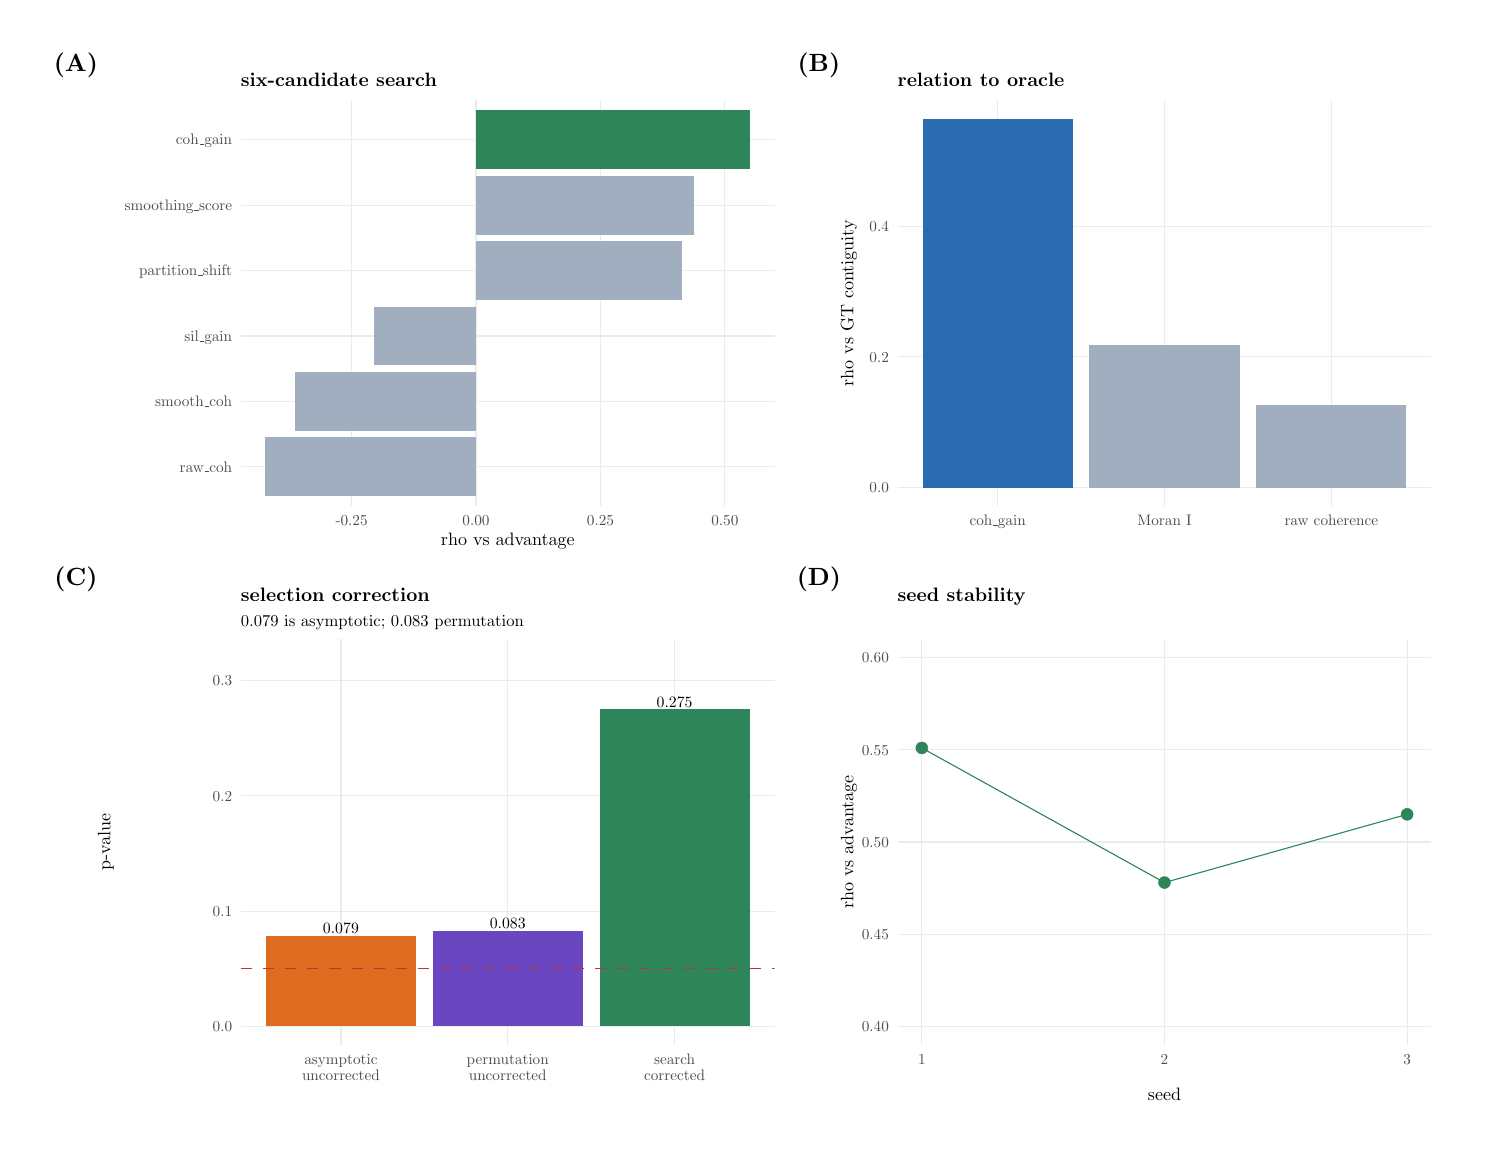
\begin{tikzpicture}[x=1pt,y=1pt]
\definecolor{fillColor}{RGB}{255,255,255}
\path[use as bounding box,fill=fillColor,fill opacity=0.00] (0,0) rectangle (516.73,397.48);
\begin{scope}
\path[clip] (  0.00,  0.00) rectangle (516.73,397.48);
\definecolor{drawColor}{RGB}{255,255,255}
\definecolor{fillColor}{RGB}{255,255,255}

\path[draw=drawColor,line width= 0.6pt,line join=round,line cap=round,fill=fillColor] (  0.00,  0.00) rectangle (516.73,397.48);
\end{scope}
\begin{scope}
\path[clip] (  5.50,206.11) rectangle (273.93,391.98);
\definecolor{fillColor}{RGB}{255,255,255}

\path[fill=fillColor] (  5.50,206.11) rectangle (273.93,391.98);
\end{scope}
\begin{scope}
\path[clip] (273.93,206.11) rectangle (511.23,391.98);
\definecolor{fillColor}{RGB}{255,255,255}

\path[fill=fillColor] (273.93,206.11) rectangle (511.23,391.98);
\end{scope}
\begin{scope}
\path[clip] (  5.50,  5.50) rectangle (273.93,206.11);
\definecolor{fillColor}{RGB}{255,255,255}

\path[fill=fillColor] (  5.50,  5.50) rectangle (273.93,206.11);
\end{scope}
\begin{scope}
\path[clip] (273.93,  5.50) rectangle (511.23,206.11);
\definecolor{fillColor}{RGB}{255,255,255}

\path[fill=fillColor] (273.93,  5.50) rectangle (511.23,206.11);
\end{scope}
\begin{scope}
\path[clip] ( 77.04,224.61) rectangle (269.93,371.19);
\definecolor{drawColor}{gray}{0.92}

\path[draw=drawColor,line width= 0.4pt,line join=round] ( 77.04,238.80) --
	(269.93,238.80);

\path[draw=drawColor,line width= 0.4pt,line join=round] ( 77.04,262.44) --
	(269.93,262.44);

\path[draw=drawColor,line width= 0.4pt,line join=round] ( 77.04,286.08) --
	(269.93,286.08);

\path[draw=drawColor,line width= 0.4pt,line join=round] ( 77.04,309.72) --
	(269.93,309.72);

\path[draw=drawColor,line width= 0.4pt,line join=round] ( 77.04,333.36) --
	(269.93,333.36);

\path[draw=drawColor,line width= 0.4pt,line join=round] ( 77.04,357.00) --
	(269.93,357.00);

\path[draw=drawColor,line width= 0.4pt,line join=round] (117.05,224.61) --
	(117.05,371.19);

\path[draw=drawColor,line width= 0.4pt,line join=round] (162.01,224.61) --
	(162.01,371.19);

\path[draw=drawColor,line width= 0.4pt,line join=round] (206.98,224.61) --
	(206.98,371.19);

\path[draw=drawColor,line width= 0.4pt,line join=round] (251.94,224.61) --
	(251.94,371.19);
\definecolor{fillColor}{RGB}{160,174,192}

\path[fill=fillColor] ( 85.80,228.16) rectangle (162.01,249.44);

\path[fill=fillColor] ( 96.46,251.80) rectangle (162.01,273.08);
\definecolor{fillColor}{RGB}{47,133,90}

\path[fill=fillColor] (162.01,346.37) rectangle (261.16,367.64);
\definecolor{fillColor}{RGB}{160,174,192}

\path[fill=fillColor] (162.01,299.08) rectangle (236.58,320.36);

\path[fill=fillColor] (125.14,275.44) rectangle (162.01,296.72);

\path[fill=fillColor] (162.01,322.72) rectangle (240.68,344.00);
\end{scope}
\begin{scope}
\path[clip] (  0.00,  0.00) rectangle (516.73,397.48);
\definecolor{drawColor}{gray}{0.30}

\node[text=drawColor,anchor=base east,inner sep=0pt, outer sep=0pt, scale=  0.55] at ( 73.89,236.90) {raw{\_{}}coh};

\node[text=drawColor,anchor=base east,inner sep=0pt, outer sep=0pt, scale=  0.55] at ( 73.89,260.54) {smooth{\_{}}coh};

\node[text=drawColor,anchor=base east,inner sep=0pt, outer sep=0pt, scale=  0.55] at ( 73.89,284.19) {sil{\_{}}gain};

\node[text=drawColor,anchor=base east,inner sep=0pt, outer sep=0pt, scale=  0.55] at ( 73.89,307.83) {partition{\_{}}shift};

\node[text=drawColor,anchor=base east,inner sep=0pt, outer sep=0pt, scale=  0.55] at ( 73.89,331.47) {smoothing{\_{}}score};

\node[text=drawColor,anchor=base east,inner sep=0pt, outer sep=0pt, scale=  0.55] at ( 73.89,355.11) {coh{\_{}}gain};
\end{scope}
\begin{scope}
\path[clip] (  0.00,  0.00) rectangle (516.73,397.48);
\definecolor{drawColor}{gray}{0.30}

\node[text=drawColor,anchor=base,inner sep=0pt, outer sep=0pt, scale=  0.55] at (117.05,217.67) {-0.25};

\node[text=drawColor,anchor=base,inner sep=0pt, outer sep=0pt, scale=  0.55] at (162.01,217.67) {0.00};

\node[text=drawColor,anchor=base,inner sep=0pt, outer sep=0pt, scale=  0.55] at (206.98,217.67) {0.25};

\node[text=drawColor,anchor=base,inner sep=0pt, outer sep=0pt, scale=  0.55] at (251.94,217.67) {0.50};
\end{scope}
\begin{scope}
\path[clip] (  0.00,  0.00) rectangle (516.73,397.48);
\definecolor{drawColor}{RGB}{0,0,0}

\node[text=drawColor,anchor=base,inner sep=0pt, outer sep=0pt, scale=  0.65] at (173.48,210.38) {rho vs advantage};
\end{scope}
\begin{scope}
\path[clip] (  0.00,  0.00) rectangle (516.73,397.48);
\definecolor{drawColor}{RGB}{0,0,0}

\node[text=drawColor,anchor=base west,inner sep=0pt, outer sep=0pt, scale=  0.70] at ( 77.04,376.05) {\bfseries six-candidate search};
\end{scope}
\begin{scope}
\path[clip] (  0.00,  0.00) rectangle (516.73,397.48);
\definecolor{drawColor}{RGB}{0,0,0}

\node[text=drawColor,anchor=base,inner sep=0pt, outer sep=0pt, scale=  0.90] at ( 17.44,381.82) {\bfseries (A)};
\end{scope}
\begin{scope}
\path[clip] (314.34,224.61) rectangle (507.23,371.19);
\definecolor{drawColor}{gray}{0.92}

\path[draw=drawColor,line width= 0.4pt,line join=round] (314.34,231.27) --
	(507.23,231.27);

\path[draw=drawColor,line width= 0.4pt,line join=round] (314.34,278.53) --
	(507.23,278.53);

\path[draw=drawColor,line width= 0.4pt,line join=round] (314.34,325.78) --
	(507.23,325.78);

\path[draw=drawColor,line width= 0.4pt,line join=round] (350.50,224.61) --
	(350.50,371.19);

\path[draw=drawColor,line width= 0.4pt,line join=round] (410.78,224.61) --
	(410.78,371.19);

\path[draw=drawColor,line width= 0.4pt,line join=round] (471.06,224.61) --
	(471.06,371.19);
\definecolor{fillColor}{RGB}{160,174,192}

\path[fill=fillColor] (383.66,231.27) rectangle (437.91,282.78);

\path[fill=fillColor] (443.94,231.27) rectangle (498.19,261.28);
\definecolor{fillColor}{RGB}{43,108,176}

\path[fill=fillColor] (323.38,231.27) rectangle (377.63,364.53);
\end{scope}
\begin{scope}
\path[clip] (  0.00,  0.00) rectangle (516.73,397.48);
\definecolor{drawColor}{gray}{0.30}

\node[text=drawColor,anchor=base east,inner sep=0pt, outer sep=0pt, scale=  0.55] at (311.19,229.38) {0.0};

\node[text=drawColor,anchor=base east,inner sep=0pt, outer sep=0pt, scale=  0.55] at (311.19,276.63) {0.2};

\node[text=drawColor,anchor=base east,inner sep=0pt, outer sep=0pt, scale=  0.55] at (311.19,323.89) {0.4};
\end{scope}
\begin{scope}
\path[clip] (  0.00,  0.00) rectangle (516.73,397.48);
\definecolor{drawColor}{gray}{0.30}

\node[text=drawColor,anchor=base,inner sep=0pt, outer sep=0pt, scale=  0.55] at (350.50,217.67) {coh{\_{}}gain};

\node[text=drawColor,anchor=base,inner sep=0pt, outer sep=0pt, scale=  0.55] at (410.78,217.67) {Moran I};

\node[text=drawColor,anchor=base,inner sep=0pt, outer sep=0pt, scale=  0.55] at (471.06,217.67) {raw coherence};
\end{scope}
\begin{scope}
\path[clip] (  0.00,  0.00) rectangle (516.73,397.48);
\definecolor{drawColor}{RGB}{0,0,0}

\node[text=drawColor,rotate= 90.00,anchor=base,inner sep=0pt, outer sep=0pt, scale=  0.65] at (298.39,297.90) {rho vs GT contiguity};
\end{scope}
\begin{scope}
\path[clip] (  0.00,  0.00) rectangle (516.73,397.48);
\definecolor{drawColor}{RGB}{0,0,0}

\node[text=drawColor,anchor=base west,inner sep=0pt, outer sep=0pt, scale=  0.70] at (314.34,376.05) {\bfseries relation to oracle};
\end{scope}
\begin{scope}
\path[clip] (  0.00,  0.00) rectangle (516.73,397.48);
\definecolor{drawColor}{RGB}{0,0,0}

\node[text=drawColor,anchor=base,inner sep=0pt, outer sep=0pt, scale=  0.90] at (285.92,381.82) {\bfseries (B)};
\end{scope}
\begin{scope}
\path[clip] ( 77.04, 29.94) rectangle (269.93,176.52);
\definecolor{drawColor}{gray}{0.92}

\path[draw=drawColor,line width= 0.4pt,line join=round] ( 77.04, 36.60) --
	(269.93, 36.60);

\path[draw=drawColor,line width= 0.4pt,line join=round] ( 77.04, 78.24) --
	(269.93, 78.24);

\path[draw=drawColor,line width= 0.4pt,line join=round] ( 77.04,119.88) --
	(269.93,119.88);

\path[draw=drawColor,line width= 0.4pt,line join=round] ( 77.04,161.53) --
	(269.93,161.53);

\path[draw=drawColor,line width= 0.4pt,line join=round] (113.20, 29.94) --
	(113.20,176.52);

\path[draw=drawColor,line width= 0.4pt,line join=round] (173.48, 29.94) --
	(173.48,176.52);

\path[draw=drawColor,line width= 0.4pt,line join=round] (233.76, 29.94) --
	(233.76,176.52);
\definecolor{fillColor}{RGB}{221,107,32}

\path[fill=fillColor] ( 86.08, 36.60) rectangle (140.33, 69.42);
\definecolor{fillColor}{RGB}{107,70,193}

\path[fill=fillColor] (146.36, 36.60) rectangle (200.61, 71.16);
\definecolor{fillColor}{RGB}{47,133,90}

\path[fill=fillColor] (206.64, 36.60) rectangle (260.89,151.12);
\definecolor{drawColor}{RGB}{197,48,48}

\path[draw=drawColor,line width= 0.4pt,dash pattern=on 4pt off 4pt ,line join=round] ( 77.04, 57.42) -- (269.93, 57.42);
\definecolor{drawColor}{RGB}{0,0,0}

\node[text=drawColor,anchor=base,inner sep=0pt, outer sep=0pt, scale=  0.57] at (113.20, 70.20) {0.079};

\node[text=drawColor,anchor=base,inner sep=0pt, outer sep=0pt, scale=  0.57] at (173.48, 71.95) {0.083};

\node[text=drawColor,anchor=base,inner sep=0pt, outer sep=0pt, scale=  0.57] at (233.76,151.90) {0.275};
\end{scope}
\begin{scope}
\path[clip] (  0.00,  0.00) rectangle (516.73,397.48);
\definecolor{drawColor}{gray}{0.30}

\node[text=drawColor,anchor=base east,inner sep=0pt, outer sep=0pt, scale=  0.55] at ( 73.89, 34.71) {0.0};

\node[text=drawColor,anchor=base east,inner sep=0pt, outer sep=0pt, scale=  0.55] at ( 73.89, 76.35) {0.1};

\node[text=drawColor,anchor=base east,inner sep=0pt, outer sep=0pt, scale=  0.55] at ( 73.89,117.99) {0.2};

\node[text=drawColor,anchor=base east,inner sep=0pt, outer sep=0pt, scale=  0.55] at ( 73.89,159.63) {0.3};
\end{scope}
\begin{scope}
\path[clip] (  0.00,  0.00) rectangle (516.73,397.48);
\definecolor{drawColor}{gray}{0.30}

\node[text=drawColor,anchor=base,inner sep=0pt, outer sep=0pt, scale=  0.55] at (113.20, 23.00) {asymptotic};

\node[text=drawColor,anchor=base,inner sep=0pt, outer sep=0pt, scale=  0.55] at (113.20, 17.06) {uncorrected};

\node[text=drawColor,anchor=base,inner sep=0pt, outer sep=0pt, scale=  0.55] at (173.48, 23.00) {permutation};

\node[text=drawColor,anchor=base,inner sep=0pt, outer sep=0pt, scale=  0.55] at (173.48, 17.06) {uncorrected};

\node[text=drawColor,anchor=base,inner sep=0pt, outer sep=0pt, scale=  0.55] at (233.76, 23.00) {search};

\node[text=drawColor,anchor=base,inner sep=0pt, outer sep=0pt, scale=  0.55] at (233.76, 17.06) {corrected};
\end{scope}
\begin{scope}
\path[clip] (  0.00,  0.00) rectangle (516.73,397.48);
\definecolor{drawColor}{RGB}{0,0,0}

\node[text=drawColor,rotate= 90.00,anchor=base,inner sep=0pt, outer sep=0pt, scale=  0.65] at ( 29.85,103.23) {p-value};
\end{scope}
\begin{scope}
\path[clip] (  0.00,  0.00) rectangle (516.73,397.48);
\definecolor{drawColor}{RGB}{0,0,0}

\node[text=drawColor,anchor=base west,inner sep=0pt, outer sep=0pt, scale=  0.60] at ( 77.04,181.18) {0.079 is asymptotic; 0.083 permutation};
\end{scope}
\begin{scope}
\path[clip] (  0.00,  0.00) rectangle (516.73,397.48);
\definecolor{drawColor}{RGB}{0,0,0}

\node[text=drawColor,anchor=base west,inner sep=0pt, outer sep=0pt, scale=  0.70] at ( 77.04,190.18) {\bfseries selection correction};
\end{scope}
\begin{scope}
\path[clip] (  0.00,  0.00) rectangle (516.73,397.48);
\definecolor{drawColor}{RGB}{0,0,0}

\node[text=drawColor,anchor=base,inner sep=0pt, outer sep=0pt, scale=  0.90] at ( 17.44,195.95) {\bfseries (C)};
\end{scope}
\begin{scope}
\path[clip] (314.34, 29.94) rectangle (507.23,176.52);
\definecolor{drawColor}{gray}{0.92}

\path[draw=drawColor,line width= 0.4pt,line join=round] (314.34, 36.60) --
	(507.23, 36.60);

\path[draw=drawColor,line width= 0.4pt,line join=round] (314.34, 69.92) --
	(507.23, 69.92);

\path[draw=drawColor,line width= 0.4pt,line join=round] (314.34,103.23) --
	(507.23,103.23);

\path[draw=drawColor,line width= 0.4pt,line join=round] (314.34,136.54) --
	(507.23,136.54);

\path[draw=drawColor,line width= 0.4pt,line join=round] (314.34,169.85) --
	(507.23,169.85);

\path[draw=drawColor,line width= 0.4pt,line join=round] (323.10, 29.94) --
	(323.10,176.52);

\path[draw=drawColor,line width= 0.4pt,line join=round] (410.78, 29.94) --
	(410.78,176.52);

\path[draw=drawColor,line width= 0.4pt,line join=round] (498.46, 29.94) --
	(498.46,176.52);
\definecolor{drawColor}{RGB}{47,133,90}

\path[draw=drawColor,line width= 0.4pt,line join=round] (323.10,137.21) --
	(410.78, 88.57) --
	(498.46,113.22);
\definecolor{fillColor}{RGB}{47,133,90}

\path[draw=drawColor,line width= 0.2pt,line join=round,line cap=round,fill=fillColor] (323.10,137.21) circle (  2.15);

\path[draw=drawColor,line width= 0.2pt,line join=round,line cap=round,fill=fillColor] (410.78, 88.57) circle (  2.15);

\path[draw=drawColor,line width= 0.2pt,line join=round,line cap=round,fill=fillColor] (498.46,113.22) circle (  2.15);
\end{scope}
\begin{scope}
\path[clip] (  0.00,  0.00) rectangle (516.73,397.48);
\definecolor{drawColor}{gray}{0.30}

\node[text=drawColor,anchor=base east,inner sep=0pt, outer sep=0pt, scale=  0.55] at (311.19, 34.71) {0.40};

\node[text=drawColor,anchor=base east,inner sep=0pt, outer sep=0pt, scale=  0.55] at (311.19, 68.02) {0.45};

\node[text=drawColor,anchor=base east,inner sep=0pt, outer sep=0pt, scale=  0.55] at (311.19,101.33) {0.50};

\node[text=drawColor,anchor=base east,inner sep=0pt, outer sep=0pt, scale=  0.55] at (311.19,134.65) {0.55};

\node[text=drawColor,anchor=base east,inner sep=0pt, outer sep=0pt, scale=  0.55] at (311.19,167.96) {0.60};
\end{scope}
\begin{scope}
\path[clip] (  0.00,  0.00) rectangle (516.73,397.48);
\definecolor{drawColor}{gray}{0.30}

\node[text=drawColor,anchor=base,inner sep=0pt, outer sep=0pt, scale=  0.55] at (323.10, 23.00) {1};

\node[text=drawColor,anchor=base,inner sep=0pt, outer sep=0pt, scale=  0.55] at (410.78, 23.00) {2};

\node[text=drawColor,anchor=base,inner sep=0pt, outer sep=0pt, scale=  0.55] at (498.46, 23.00) {3};
\end{scope}
\begin{scope}
\path[clip] (  0.00,  0.00) rectangle (516.73,397.48);
\definecolor{drawColor}{RGB}{0,0,0}

\node[text=drawColor,anchor=base,inner sep=0pt, outer sep=0pt, scale=  0.65] at (410.78,  9.76) {seed};
\end{scope}
\begin{scope}
\path[clip] (  0.00,  0.00) rectangle (516.73,397.48);
\definecolor{drawColor}{RGB}{0,0,0}

\node[text=drawColor,rotate= 90.00,anchor=base,inner sep=0pt, outer sep=0pt, scale=  0.65] at (298.39,103.23) {rho vs advantage};
\end{scope}
\begin{scope}
\path[clip] (  0.00,  0.00) rectangle (516.73,397.48);
\definecolor{drawColor}{RGB}{0,0,0}

\node[text=drawColor,anchor=base west,inner sep=0pt, outer sep=0pt, scale=  0.70] at (314.34,190.18) {\bfseries seed stability};
\end{scope}
\begin{scope}
\path[clip] (  0.00,  0.00) rectangle (516.73,397.48);
\definecolor{drawColor}{RGB}{0,0,0}

\node[text=drawColor,anchor=base,inner sep=0pt, outer sep=0pt, scale=  0.90] at (285.92,195.95) {\bfseries (D)};
\end{scope}
\end{tikzpicture}
